\chapter{IDS Implementation}

Let's get serious now! An overview of IDS and how statistical techniques can be used with it has been proposed the next step is how to make all these things working together and what are the problems when you go from theory to practice!\newline\newline
In this example, it has been used the KDDCUP99 dataset, a well known set of network data collected by a military company\newline
The steps one must follow in order to build a good system, both in intrusion detection efficiency and computational efficiency are the followings:
\begin{itemize}
	\item[1)] \textbf{Data preprocess} - In this step the main issue is that most of the times data are numbers and strings mixed together. A numerical representation for all the strings in the dataset is mandatory for the next steps
	\item[2)] \textbf{Data standardization/normalization} - At this point, if we observe the dataset D, it can be seen that the range of numbers in D is not uniform. What must be done here is to run an algorithm that produces an output consisting of a new dataset D' where the values are standardized (or normalized, according to your needs)
	\item[3)] \textbf{Decision Tree method} Last step. The classification tool (the Decision Tree in this case) must be fed with the new dataset D' to build the data structure that will be then used to detect intrusions and malicious behaviours
\end{itemize}

A visual model for these steps is given in the next figure.

\begin{figure}[h!]
	\centering
	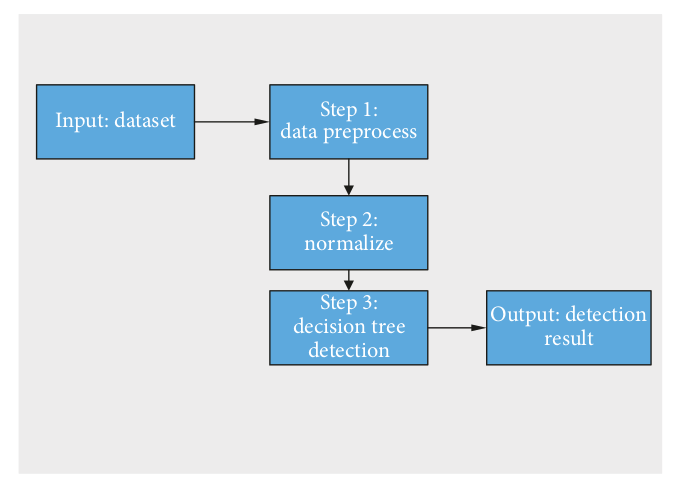
\includegraphics[width=\textwidth]{img/Steps.png}
\end{figure}

\begin{minipage}{\linewidth}
\vspace{0.5cm}
So, the first step is to preprocess data in order to work with them. This step is nothing but technical and requires really little skills

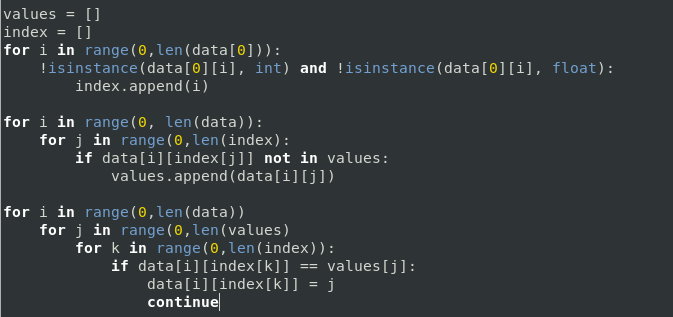
\includegraphics[width=\textwidth]{img/PreprocessCode.png}

\end{minipage}

\vspace{0.5cm}

At this point, there is the need to standardize the data in order to be able to do the Principal Component Analysis. This is a very important step because, if wrongly implemented, it can really blast down the accuracy of predictions.\newline
Standardizing data mean that the new dataset must have all the distributions associated to the features with mean = 0 and variance = 1.\newline\newline
Luckily, there is a python library that implements a lot of these features for us: the Pandas library.\newline\newline
The very important drawback here is that we can't standardize the train-set and the test-set separately (or the accuracy of prediction will be mined): the train-set must be standardized first and the same criteria must be used to standardize the test-set as well. In other words: the scaler must be "fit" using the train-set and then use the \emph{same} scaler to apply the transformation to both sets\newline\newline
\vspace{0.3cm}
\begin{minipage}{\linewidth}

	\centering
	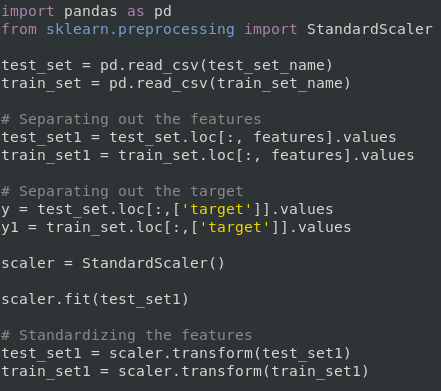
\includegraphics[width=\textwidth]{img/Normalization.png}
\end{minipage}

\vspace{0.5cm}

\begin{minipage}{\linewidth}
At this point, Principal Component Analysis algorithm can be run in order to exclude those features that have little significance for our purpose:\newline\newline

	\centering
	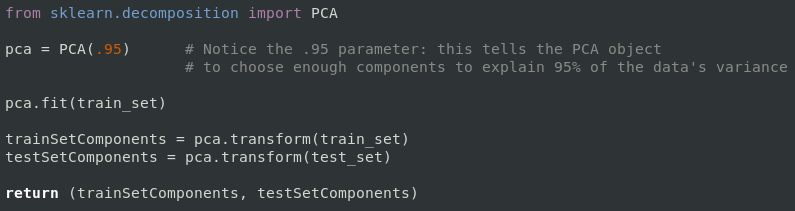
\includegraphics[width=\textwidth]{img/PCA.png}
	
	\vspace{0.5cm}

Now that data have been cleaned, standardized, and the features reduced those that are the most relevant, they can be used to feed the Decision Tree algorithm!\newline\newline
For the Tree construction the \emph{rpart} package has been used, due to its acceptance in statistical/machine learning environments. It is also quite efficient and let the user specify a lot of useful parameters for the tree construction.\newline In the next few lines, the algorithm used to build a Decision Tree is briefly described:

\begin{itemize}
	\item[1)] For each variable the whole dataset is split in 2 parts, using the Gini Index
		\begin{itemize}
			\item[$\rightarrow$] Since the variables are somehow continuous, splits will be done on boolean conditions: given a \emph{threshold t} features will be split according to the ones greater than \emph{t}, or lower than \emph{t}
		\end{itemize}
	\item[2)] The variable (or feature) that produced the highest score (the lowest Gini Index) will be the very first split of the Tree (the root node)
	\item[3)] The algorithm now proceeds recursively on each node, until there are no more variable to split
\end{itemize}

	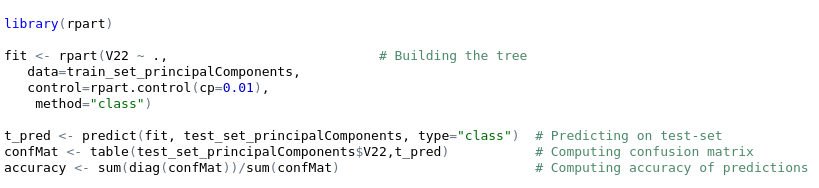
\includegraphics[width=\textwidth]{img/Rpart.png}
	
\end{minipage}

\vspace{0.5cm}

\begin{minipage}{\linewidth}

	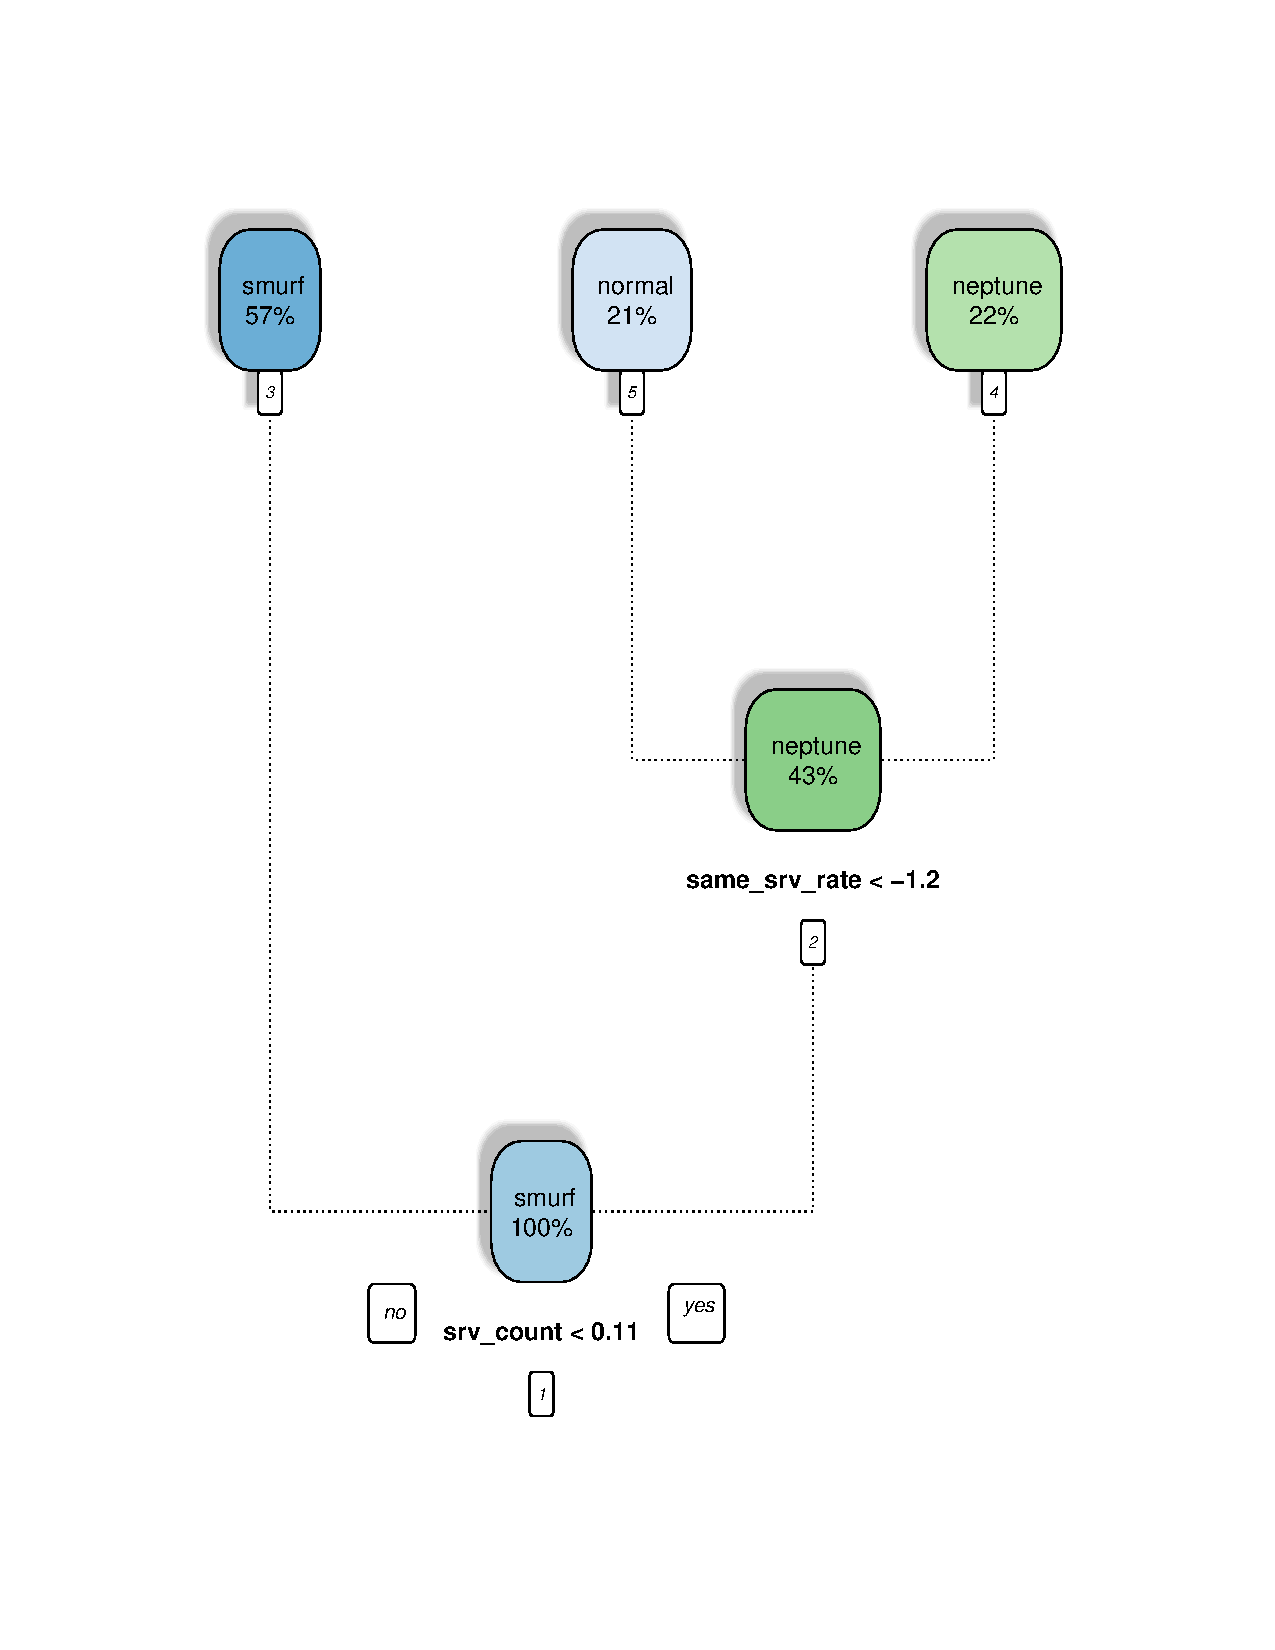
\includepdf{img/RplotStupido.pdf}
	Small and simple tree example to be read bottom-up
	
\end{minipage}
	